% !TeX root = ../../../main.tex
\begin{figure}[htbp]
\begin{ChFiveFloatBody}
\centering
    % \begin{minipage}{0.45\textwidth}
        % \centering
        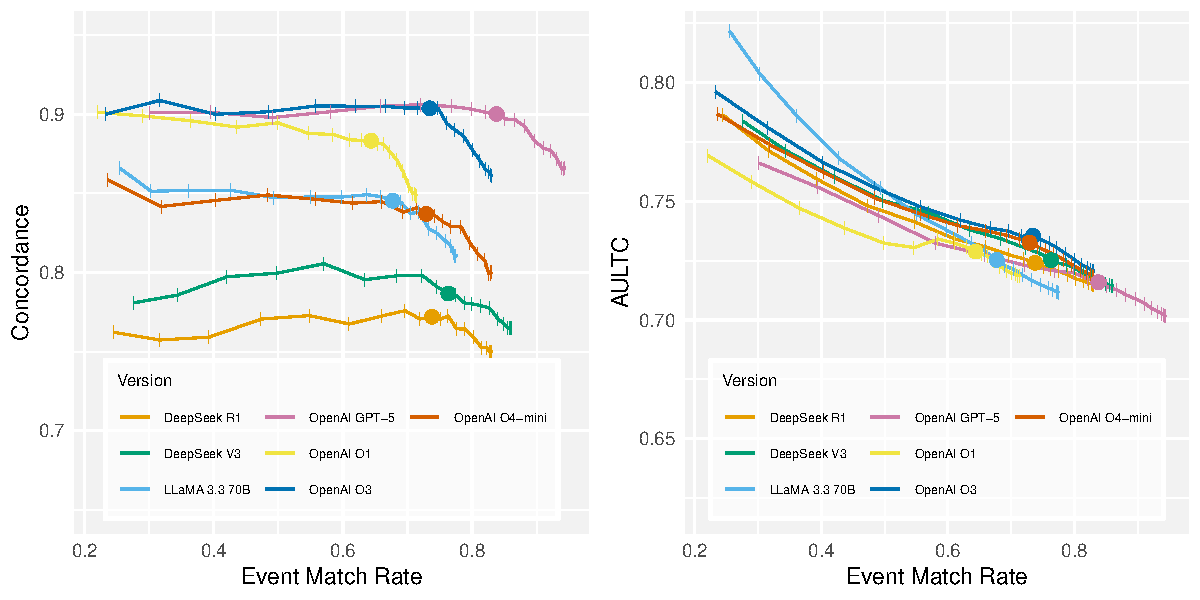
\includegraphics[width=\linewidth]{Chapters/chapter-05/images/Scientific_data/Plots_tables/event_match_vs_metrics_updated.pdf}
        % \caption{}
    % \end{minipage}
    % \hfill
    % \begin{subfigure}[t]{\linewidth}
    %     \centering
    %     \includegraphics[width=\linewidth]{Plots_tables/event_match_vs_metrics_updated.pdf}
    %     \caption{Concordance and AULTC by event match rate (\textbf{recursive matching heuristic}).}
    %     \label{ch05:fig:threshold_tradeoff_greedy}
    % \end{subfigure}

    % \begin{subfigure}[t]{\linewidth}
    %     \centering
    %     \includegraphics[width=\linewidth]{Plots_tables/event_match_vs_metrics_lapjv.pdf}
    %     \caption{Concordance and AULTC by event match rate (\textbf{LAPJV matching).}}
    %     \label{ch05:fig:threshold_tradeoff_greedy}
    % \end{subfigure}
    
    
    

\end{ChFiveFloatBody}
\caption{Concordance and AULTC by event match rate for recursive matching heuristic. Solid circle ($\bullet$) represents threshold of 0.1, with ticks (|) indicating 0.01 increments of the threshold in [0.01, 0.50].
    }\ChFiveFloatLabel{ch05:fig:threshold_tradeoff_greedy}
\end{figure}